\chapter{Ewaluacja zaimplementowanych algorytmów}
\label{cha:ewaluacja}

\section{Metodologia przeprowadzonych testów}
\label{sec:metodologia_testow}

Testy algorytmów zaimplementowanych w Laboratorium Biocybernetyki AGH zostały przeprowadzone zgodnie z metodologią opisaną w \cite{changedetection_15}. 
%%TODO one nie zostały opracowane na AGH...
Sekwencje testowe pochodzą z bazy \textit{ChangeDetection} \cite{change_detection_web}. 
Tego typu podejście do ewaluacji zaimplementowanych algorytmów zostało wykorzystane między innymi w~\cite{kryjak_14_vibe, kryjak_14_pbas, janus_15}. 
Wszystkie metody zostały przetestowane z wykorzystaniem 31 sekwencji testowych podzielonych na 6 różnych kategorii. 
Zbiór testowy został tak dobrany, aby odwzorować jak największą liczbę sytuacji mogących wystąpić w rzeczywistych warunkach. %%TODO środowisku czego ?
Każda z kategorii została szczegółowo opisana w rozdziale \ref{sec:testy}. Wszystkie testy przeprowadzono z wykorzystaniem modeli programowych, opisanych w rozdziale \ref{sec:modele_programowe}.

Dla każdej sekwencji testowej zawartej w bazie, dostępny jest model wzorcowy tj. ręcznie anotowana maska obiektów (ang. \textit{ground truth}).
Wzorzec zapisany jest jako obraz w skali szarości, gdzie piksele przyjmują jedną z pięciu wartości:

\begin{eqwhere}[2cm]
	\item[$0$] tło
	\item[$50$] cienie
	\item[$85$] obszar wyłączony z analizy
	\item [$175$] obszar trudny do zidentyfikowania (np. kontur otaczający ruchomy obiekt)
	\item [$255$] obiekt pierwszoplanowy \\
\end{eqwhere}  

\noindent Porównując ramki wyjściowe testowanego algorytmu z odpowiadającymi im ramkami modelu wzorcowego, można wyznaczyć następujące współczynniki:
\begin{eqwhere}[2cm]
	\item[$\small TP$] liczba pikseli poprawnie zakwalifikowanych jako pierwszy plan (ang. \textit{true positive})
	\item[$\small TN$] liczba pikseli poprawnie zakwalifikowanych jako tło (ang. \textit{true negative})
	\item[$\small FN$] liczba pikseli błędnie zakwalifikowanych jako tło (ang. \textit{false negative})
	\item[$\small FP$] liczba pikseli błędnie zakwalifikowanych jako pierwszy plan (ang. \textit{false positive})\\
\end{eqwhere}

\noindent Na podstawie wyznaczonych współczynników oblicza się 7 wskaźników jakości określających dokładność metody:
%
\TabPositions{0.45\linewidth}
\begin{enumerate}[nolistsep]
	\item \textit{Recall (Re)} : \tab \small{$TP/(TP+FN)$}
	\item \textit{Specificity (Spec)} : \tab \small{$TN/(TN+FP)$}
	\item \textit{False Positive Rate (FPR)} : \tab \small{$FP/(FP + TN)$}
	\item \textit{False Negative Rate (FNR)} : \tab \small{$FN/(FN + TP)$}
	\item \textit{Percentage of Wrong Classifications (PWC)} : \tab \small{$100(FN + FP)/(TP + FN + FP + TN)$}
	\item \textit{Precision (Pr)} : \tab \small{$TP/(TP + FP)$}
	\item \textit{F-measure (F1)} : \tab \small{$2\frac{P_r*R_e}{P_r+R_r}$}\\
\end{enumerate}

Parametr \textit{Re} definiuje jaki procent pikseli pierwszoplanowych został rozpoznany. 
Analogiczną wartość dla pikseli reprezentujących tło określa parametr \textit{Se}. 
Parametry \textit{FPR} i \textit{FNR} są przeciwieństwem wartości opisanych wyżej i wynoszą odpowiednio $1-Se$ i $1-Re$. 
\textit{PWC} określa procent źle sklasyfikowany pikseli, natomiast \textit{Pr} informuje jaki procent spośród pikseli sklasyfikowanych jako pierwszoplanowe został rozpoznany prawidłowo.
%TODO zdanie o F1

\section{Szczegółowe testy}
\label{sec:testy}
%%TODO test -> testy ?

\subsection{Sekwencje podstawowe}
\label{subsec:sewkencje_podstawowe}

W pierwszej kolejności dokonano porównania algorytmów przy użyciu sekwencji testowych z kategorii \textit{Baseline}. 
Wykorzystano 4 sekwencje, z czego dwie nagrano na otwartej przestrzeni i dwie w~zamkniętym pomieszczeniu. 
Przykładowa sekwencja została pokazana na rysunku \ref{fig:baseline_example}. 
Jest to zdecydowanie najprostsza spośród wszystkich kategorii i jednocześnie najbardziej zróżnicowana. 
Dzięki temu może stanowić dobry punkt odniesienia dla dalszych testów. 
Dwie spośród wykorzystanych sekwencji zawierają głównie obiekty ruchome, natomiast w dwóch kolejnych występują także obiekty zatrzymane. 
Oprócz tego miejscami pojawiają się cienie oraz dynamiczne tło. 
Szczegółowe wyniki wykonanych testów przedstawiono w tabeli \ref{tab:baseline}.
%%TODO dla jakich parametrów, napisać czy to były modele programowe czy co ? floating, fixed itp ? - pierwszy akapit

    \begin{figure}[h]
			\centering
			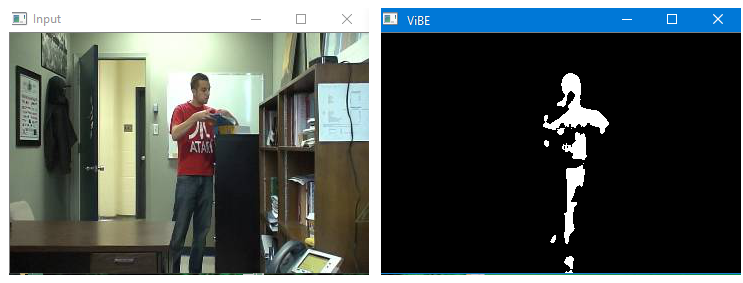
\includegraphics[scale=0.8]{img/5/baseline_example.png}
			\caption{Sekwencja \textit{office} z kategorii \textit{Baseline}}
			\label{fig:baseline_example}
	\end{figure}

	\begin{table}[h]
		\centering
		\begin{threeparttable}
			\caption{Średnie rezultaty uzyskane dla sekwencji z kategorii \textit{Baseline}}
			\label{tab:baseline}
	\small{
			\begin{tabular}{| R{3cm} || m{1cm} | m{1cm} | m{1cm} | m{1cm} | m{1cm} | m{1cm} | m{1cm} |}  
			\hline
			 & \multicolumn{1}{l|}{\textit{Recall}} & \multicolumn{1}{l|}{\textit{Spec}} & \multicolumn{1}{l|}{\textit{FPR}}
			 & \multicolumn{1}{l|}{\textit{FNR}} & \multicolumn{1}{l|}{\textit{PWC}} & \multicolumn{1}{l|}{\textit{F1}} & \multicolumn{1}{l|}{\textit{Prec}} \\
			\hline \hline
			\textit{metoda naiwna} & \num{0.8630} & \num{0.9973} & \num{0.0027} & \num{0.1370} & \num{0.68} & \num{0.8918} & \num{0.9237} \\
			\hline
			\textit{odejmowanie ramek} & \num{0.2567} & \num{0.9988} & \num{0.0012} & \num{0.7433} & \num{3.06} & \num{0.3521} & \num{0.8352} \\
			\hline
			\textit{średnia krocząca} & \num{0.6594} & \num{0.9797} & \num{0.0203} & \num{0.3406} & \num{3.62} & \num{0.4828} & \num{0.4685} \\
			\hline
			\textit{ViBE} & \num{0.8871} & \num{0.9977} & \num{0.0023} & \num{0.1129} & \num{0.64} & \num{0.9126} & \num{0.9403} \\
			\hline
            \textit{PBAS} & \num{0.7457} & \num{0.9978} & \num{0.0022} & \num{0.2543} & \num{1.23} & \num{0.8084} & \num{0.9109} \\
			\hline
			\textit{PBAS+} & \num{0.9075} & \num{0.9965} & \num{0.0035} & \num{0.0925} & \num{0.58} & \num{0.8998} & \num{0.8932} \\
			\hline 		
			\textit{GMM} & \num{0.5235} & \num{0.9703} & \num{0.0296} & \num{0.4764} & \num{5.32} & \num{0.5376} & \num{0.5604} \\
			\hline
			\end{tabular}
			}		
		\end{threeparttable}
	\end{table}

Spośród prostych algorytmów, zdecydowanie najlepszy wynik uzyskano przy wykorzystaniu metody naiwnej. 
Odejmowanie ramek oraz średnia krocząca zwracają już zdecydowanie gorsze rezultaty. 
Jak zostało już wspomniane w części teoretycznej (rozdział \ref{sec:proste_metody}), są to algorytmy nadające się głównie do detekcji obiektów ruchomych, stąd też zdecydowanie gorszy wynik. %%TODO brak ref
Dla większości testowanych algorytmów można zaobserwować stosunkowo wysoką wartość wskaźników \textit{Spec} i \textit{Prec} oraz niewielką wartość \textit{PWC}, co oznacza bardzo dobrą eliminację szumów. 

Wartym uwagi jest fakt, że dla standardowej wersji algorytmu \textit{PBAS} otrzymano gorsze wartości wskaźników niż dla metody \textit{ViBE}. 
W testowanych sekwencjach występowały również obiekty zatrzymane, które w przypadku obu wspomnianych metod często zostawały wtapiane w tło, świadczy o tym stosunkowo niska wartość wskaźnika \textit{recall}. 
Problem ten nie został zaobserwowany dla rozszerzonej wersji algorytmu \textit{PBAS} (oznaczonej jako \textit{PBAS+}), w której wykorzystano dodatkowy mechanizm detekcji obiektów statycznych. 
Wskaźniki jakości otrzymane dla algorytmu \textit{GMM} są z kolei niższe niż dla omówionych wyżej właśnie algorytmów, ale również wyraźnie lepsze niż dla najprostszej metody odejmowania ramek i średniej kroczącej. 


\subsection{Dynamiczne tło i cienie}
\label{subsec:dynamiczne_tlo_cienie}

Kategoria \textit{Dynamic Background} składa się z 6 sekwencji zawierających dynamiczne tło. 
Występuje ono pod różnymi formami, takimi jak fale na wodzie, fontanna oraz gałęzie z liśćmi poruszające się pod wpływem wiatru. 
Przykładowy kadr z takiej sekwencji zamieszczono na rysunku \ref{fig:dynamic_example}. 
Druga z omawianych kategorii to \textit{Shadows}. 
Również zawiera 6 sekwencji, w których głównym utrudnieniem dla algorytmów segmentacji tła są licznie występujące cienie. 
Otrzymane dla poszczególnych algorytmów rezultaty zamieszczono tabelach \ref{tab:dynamic_background} (kategoria \textit{Dynamic Background}) oraz \ref{tab:shadows} (kategoria \textit{Shadows}).

    \begin{figure}[h]
			\centering
			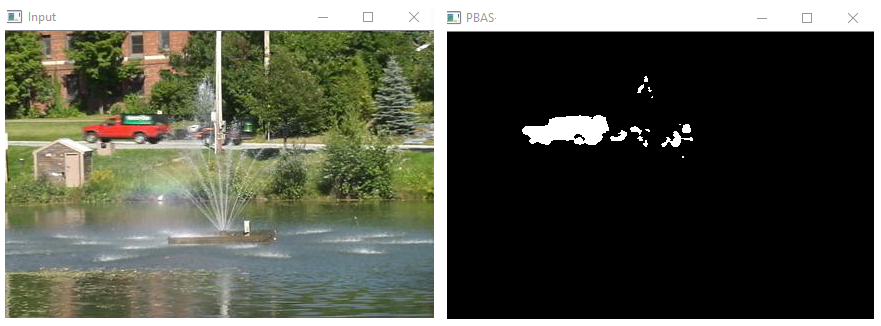
\includegraphics[scale=0.65]{img/5/dynamic_example.png}
			\caption{Sekwencja \textit{fountain02} z kategorii \textit{Dynamic Background}}
			\label{fig:dynamic_example}
	\end{figure}

	\begin{table}[h]
		\centering
		\begin{threeparttable}
			\caption{Średnie rezultaty uzyskane dla sekwencji z kategorii \textit{Dynamic Background}}
			\label{tab:dynamic_background}
	\small{
			\begin{tabular}{| R{3cm} || m{1cm} | m{1cm} | m{1cm} | m{1cm} | m{1cm} | m{1cm} | m{1cm} |}  
			\hline
			 & \multicolumn{1}{l|}{\textit{Recall}} & \multicolumn{1}{l|}{\textit{Spec}} & \multicolumn{1}{l|}{\textit{FPR}}
			 & \multicolumn{1}{l|}{\textit{FNR}} & \multicolumn{1}{l|}{\textit{PWC}} & \multicolumn{1}{l|}{\textit{F1}} & \multicolumn{1}{l|}{\textit{Prec}} \\
			\hline \hline
			\textit{metoda naiwna} & \num{0.7994} & \num{0.9603} & \num{0.0397} & \num{0.2006} & \num{4.0673} & \num{0.3819} & \num{0.2866} \\
			\hline
			\textit{odejmowanie ramek} & \num{0.2841} & \num{0.9913} & \num{0.0087} & \num{0.7159} & \num{1.8137} & \num{0.2848} & \num{0.6162} \\
			\hline
			\textit{średnia krocząca} & \num{0.6736} & \num{0.9605} & \num{0.0395} & \num{0.3264} & \num{4.3561} & \num{0.3308} & \num{0.2593} \\
			\hline
			\textit{ViBE} & \num{0.8108} & \num{0.9877} & \num{0.0123} & \num{0.1892} & \num{1.3591} & \num{0.6652} & \num{0.6748} \\
			\hline
            \textit{PBAS} & \num{0.4749} & \num{0.9980} & \num{0.0020} & \num{0.5251} & \num{0.9153} & \num{0.5325} & \num{0.7776} \\
			\hline
			\textit{PBAS+} & \num{0.9396} & \num{0.9748} & \num{0.0252} & \num{0.0604} & \num{2.5478} & \num{0.6187} & \num{0.5567} \\
			\hline 		
			\textit{GMM} & \num{0.5467} & \num{0.9428} & \num{0.0572} & \num{0.4533} & \num{6.2624} & \num{0.2669} & \num{0.2009} \\
			\hline
			\end{tabular}
			}		
		\end{threeparttable}
	\end{table}

W przedstawionych algorytmach nie zastosowano żadnych dodatkowych mechanizmów wspomagających wykrywanie dynamicznego tła oraz cieni. 
Po raz kolejny stosunkowo dobre wyniki, jak na prostotę tego algorytmu, uzyskano dla metody naiwnej. 
Dla większości algorytmów, podczas testów w~kategorii \textit{dynamic background} uzyskano wysoką wartość wskaźnika \textit{recall}, co oznacza dokładną detekcję rzeczywistych obiektów pierwszoplanowych. 
Słaby rezultat, zgodnie z oczekiwaniami, otrzymano w przypadku metody odejmowania ramek. 
Wyniki niższe od pozostałych uzyskano również dla algorytmów \textit{GMM} i \textit{PBAS}, z kolei najwyższy wskaźnik otrzymano dla rozszerzonej wersji metody \textit{PBAS+}.

Niestety w większości przypadków uzyskano również zdecydowanie niższą wartość wskaźnika \textit{Prec} i \textit{PWC}, co oznacza, że dynamicznie poruszające się elementy w tle zostały mylnie zaklasyfikowane jako pierwszy plan. 
Szczególnie widoczne jest to dla metody naiwnej, natomiast najlepiej pod tym względem wypadły algorytmy \textit{ViBE} oraz \textit{PBAS}. 
Warto zaznaczyć, że rozszerzona wersja metody \textit{PBAS} charakteryzuje się zdecydowanie słabszą zdolnością wyodrębniania dynamicznego tła od statycznego planu, jednak zapewnia lepszą dokładność w wykrywaniu prawdziwych obiektów pierwszoplanowych (wyższa wartość wskaźnika \textit{recall}).
%TODO a może Pan przemyśleć dlaczego tak się dzieje ?

	\begin{table}[h]
		\centering
		\begin{threeparttable}
			\caption{Średnie rezultaty uzyskane dla sekwencji z kategorii \textit{Shadows}}
			\label{tab:shadows}
	\small{
			\begin{tabular}{| R{3cm} || m{1cm} | m{1cm} | m{1cm} | m{1cm} | m{1cm} | m{1cm} | m{1cm} |}  
			\hline
			 & \multicolumn{1}{l|}{\textit{Recall}} & \multicolumn{1}{l|}{\textit{Spec}} & \multicolumn{1}{l|}{\textit{FPR}}
			 & \multicolumn{1}{l|}{\textit{FNR}} & \multicolumn{1}{l|}{\textit{PWC}} & \multicolumn{1}{l|}{\textit{F1}} & \multicolumn{1}{l|}{\textit{Prec}} \\
			\hline \hline
			\textit{metoda naiwna} & \num{0.8253} & \num{0.9686} & \num{0.0314} & \num{0.1747} & \num{3.7359} & \num{0.6603} & \num{0.6129} \\
			\hline
			\textit{odejmowanie ramek} & \num{0.1809} & \num{0.9970} & \num{0.0030} & \num{0.8191} & \num{3.7981} & \num{0.2700} & \num{0.7968} \\
			\hline
			\textit{średnia krocząca} & \num{0.5992} & \num{0.9551} & \num{0.0449} & \num{0.4008} & \num{6.0793} & \num{0.4864} & \num{0.4436} \\
			\hline
			\textit{ViBE} & \num{0.8738} & \num{0.9891} & \num{0.0109} & \num{0.1262} & \num{1.5202} & \num{0.8212} & \num{0.7884} \\
			\hline
            \textit{PBAS} & \num{0.6152} & \num{0.9889} & \num{0.0111} & \num{0.3848} & \num{2.7448} & \num{0.6739} & \num{0.7951} \\
			\hline
			\textit{PBAS+} & \num{0.8590} & \num{0.9881} & \num{0.0119} & \num{0.1410} & \num{1.8909} & \num{0.7903} & \num{0.7479} \\
			\hline 		
			\textit{GMM} & \num{0.5478} & \num{0.9949} & \num{0.0051} & \num{0.4522} & \num{3.2416} & \num{0.6605} & \num{0.8510} \\
			\hline
			\end{tabular}
			}		
		\end{threeparttable}
	\end{table}

Testy w kategorii \textit{shadows} pokazały, że mimo braku osobnego mechanizmu do detekcji i eliminacji cieni, podobnie jak w przypadku poprzedniego testu, wyniki są satysfakcjonujące. 
Również w tym przypadku metoda naiwna zwraca bardzo dobre rezultaty, zarówno pod względem liczby wykrytych obiektów (parametr \textit{recall}) jak i dokładności (parametry \textit{PWC} i \textit{prec}). 
Ponownie można zaobserwować wyraźną różnicę pomiędzy podstawową i rozszerzoną wersją algorytmu \textit{PBAS} oraz bardzo dobry wynik metody \textit{ViBE}. 
W przypadku tego testu algorytm \textit{GMM} charakteryzuje się bardzo wysoką precyzją, jednak przy zdecydowanie za niskim poziomie rozpoznawalności obiektów.

\subsection{Drgania kamery}
\label{subsec:drgania_kamery}

W kategorii \textit{Camera Jitter} zawierają się 4 sekwencje testowe, w których kamera nieustannie poddawana jest lekkim oraz silniejszym wibracjom. 
Poziom wibracji jest zróżnicowany dla poszczególnych sekwencji. 
Przykładową sekwencję zamieszczono na rysunku \ref{fig:jitter_example}, natomiast uzyskane rezultaty przedstawiono w tabeli \ref{tab:camera_jitter}. 

    \begin{figure}[h]
			\centering
			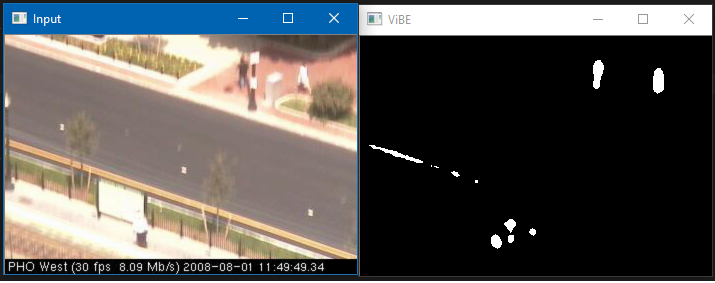
\includegraphics[scale=0.8]{img/5/jitter_example.png}
			\caption{Sekwencja \textit{boulevard} z kategorii\textit{Camera Jitter}}
			\label{fig:jitter_example}
	\end{figure}

	\begin{table}[h]
		\centering
		\begin{threeparttable}
			\caption{Średnie rezultaty uzyskane dla sekwencji z kategorii \textit{Camera Jitter}}
			\label{tab:camera_jitter}
	\small{
			\begin{tabular}{| R{3cm} || m{1cm} | m{1cm} | m{1cm} | m{1cm} | m{1cm} | m{1cm} | m{1cm} |}  
			\hline
			 & \multicolumn{1}{l|}{\textit{Recall}} & \multicolumn{1}{l|}{\textit{Spec}} & \multicolumn{1}{l|}{\textit{FPR}}
			 & \multicolumn{1}{l|}{\textit{FNR}} & \multicolumn{1}{l|}{\textit{PWC}} & \multicolumn{1}{l|}{\textit{F1}} & \multicolumn{1}{l|}{\textit{Prec}} \\
			\hline \hline
			\textit{metoda naiwna} & \num{0.6797} & \num{0.8546} & \num{0.1454} & \num{0.3203} & \num{15.0577} & \num{0.2906} & \num{0.1884} \\
			\hline
			\textit{odejmowanie ramek} & \num{0.4640} & \num{0.8746} & \num{0.1254} & \num{0.5360} & \num{14.1708} & \num{0.2134} & \num{0.1408} \\
			\hline
			\textit{średnia krocząca} & \num{0.7625} & \num{0.8487} & \num{0.1513} & \num{0.2375} & \num{15.2717} & \num{0.3205} & \num{0.2091} \\
			\hline
			\textit{ViBE} & \num{0.7510} & \num{0.9371} & \num{0.0629} & \num{0.2490} & \num{6.9322} & \num{0.5119} & \num{0.3964} \\
			\hline
			\textit{ViBE+} & \num{0.7510} & \num{0.9371} & \num{0.0629} & \num{0.2490} & \num{6.9322} & \num{0.5119} & \num{0.3964} \\
			\hline
            \textit{PBAS} & \num{0.6523} & \num{0.9843} & \num{0.0157} & \num{0.3477} & \num{2.7535} & \num{0.6416} & \num{0.6382} \\
			\hline
			\textit{PBAS+} & \num{0.8907} & \num{0.8889} & \num{0.1111} & \num{0.1093} & \num{11.0708} & \num{0.4072} & \num{0.2697} \\
			\hline 		
			\textit{GMM} & \num{0.5998} & \num{0.9098} & \num{0.0902} & \num{0.4002} & \num{10.7799} & \num{0.4128} & \num{0.3210} \\
			\hline
			\end{tabular}
			}		
		\end{threeparttable}
	\end{table}
	
Oprócz testowanych wcześniej algorytmów, w tym przypadku ewaluacji poddano także rozszerzoną wersje metody \textit{ViBE}, zawierającą dodatkowy mechanizm redukcji efektu ruchomej kamery. 
Niestety, zaimplementowane rozwiązanie nie zdało egzaminu i dla wykorzystanych sekwencji testowych uzyskany wynik jest niezadowalający. Według autorów algorytm został przygotowany z myślą o zastosowaniu w kamerach typu \textit{PTZ} (ang. \textit{pan–tilt–zoom camera}). Wymagania systemu działającego z tego typu urządzeniem częściowo pokrywają się z tym czego wymagamy od algorytmu redukującego drgania kamery. W związku z tym zdecydowano się przetestować zaproponowane rozwiązanie właśnie w takim środowisku, uwzględniając jednak, że docelowe zastosowanie było inne, uzyskanego wyniku nie należy traktować jak niespełniającego wymagań.
%Implementacja algorytmu została przygotowana z myślą o pracy w rzeczywistym środowisku i w rozdzielczości \textit{576p@50fps}. 
%W przypadku przeprowadzanych testów obraz wejściowy jest dużo gorszej jakości. 
%Opracowana koncepcja obliczania przepływu optycznego, zakładająca dzielenie obrazu na równe bloki o rozmiarze $32x32$ nie daje akceptowalnych rezultatów dla niższych rozdzielczości. 
%%TODO analizował Pan to jakoś bardziej ? Jak tak to proszę jeszcze to rozwinąć.
Pozostałe algorytmy uzyskały niskie wartości wskaźnika \textit{prec} oraz wysoki procent źle sklasyfikowanych pikseli (\textit{PWC}). 
Jest to naturalny efekt drgań kamery, ponieważ w takim przypadku niemal cały obraz interpretowany jest jako pierwszy plan.

%%TODO z tego co pamiętam... to był raczej płynny ruch kamery a nie wprost drgania. Zatem może też o to chodzi...
%%TODO bo to ogolnie miało być do takiej kamery PTZ
Przygotowana implementacja algorytmu \textit{ViBE}, została początkowo opracowana w Laboratorium Biocybernetyki AGH i po raz pierwszy opublikowana w artykule \cite{kryjak_14_vibe}. 
Autorzy tej publikacji zaproponowali alternatywny sposób przetestowania przygotowanego rozwiązania. 
Koncepcja ta zakłada testowanie metody w rzeczywistych warunkach, w trzech różnych sytuacjach oznaczanych dalej jako \textit{C1, C2, C3}:\\
\-\hspace{1cm} $C1$ -- brak obiektów pierwszoplanowych, jedynie ruch kamery\\
\-\hspace{1cm} $C2$ -- poruszające się obiekty pierwszoplanowe oraz ruchoma kamera\\
\-\hspace{1cm} $C3$ -- pojawia się obiekt zatrzymany, następnie kamera zaczyna się ruszać\\
\\
\noindent Działanie algorytmu w takim środowisku zilustrowano na rysunku \ref{fig:vibe_jitter_real}, natomiast otrzymane wyniki z przeprowadzonych w ten sposób testów zamieszczono w tabeli \ref{tab:vibe_real}.

	\begin{figure}[h]
		\centering
		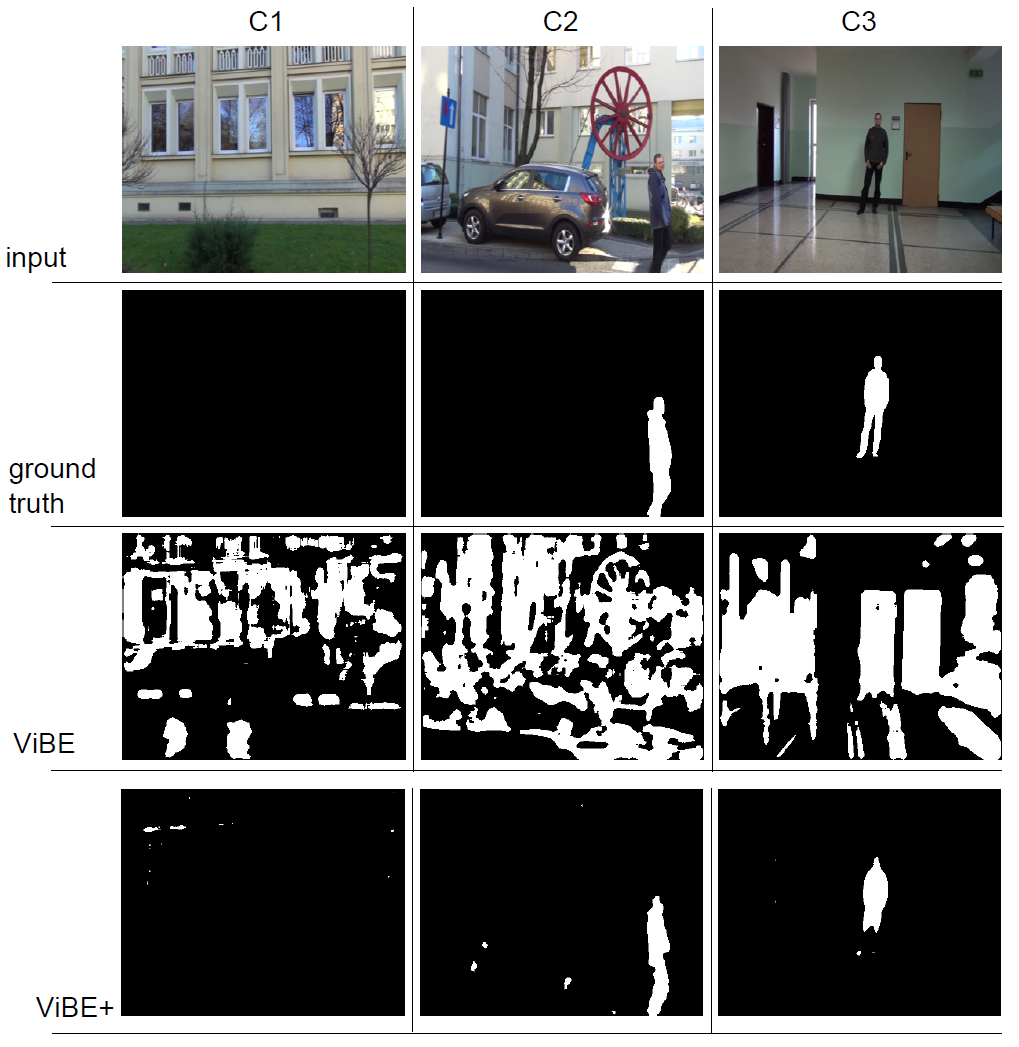
\includegraphics[scale=0.5]{img/5/vibe_real_test.png}
		\caption{Działanie algorytmu \textit{ViBE} w rzeczywistym środowisku -- źródło \cite{kryjak_14_vibe}}
		\label{fig:vibe_jitter_real}
	\end{figure}

	\begin{table}[h]
		\centering
		\begin{threeparttable}
			\caption{Testy algorytmu \textit{ViBE} w rzeczywistym środowisku -- źródło \cite{kryjak_14_vibe}}
			\label{tab:vibe_real}
	\small{
			\begin{tabular}{| R{1cm} | m{1cm} | m{1cm} | m{1cm} | m{1cm} | m{1cm} |}  
			\hline
			 \multicolumn{1}{|l|}{\textit{Kategoria}} &  \multicolumn{1}{l|}{\textit{Algorytm}} & \multicolumn{1}{l|}{\textit{Recall}} & \multicolumn{1}{l|}{\textit{PWC}} & \multicolumn{1}{l|}{\textit{F1}} & \multicolumn{1}{l|}{\textit{Prec}} \\
			\hline \hline
            \multirow{2}{*}{\textit{C1}} & \textit{ViBE} & -- & \num{36.66} & -- & \num{0.0} \\
			& \textit{ViBE+} & -- & \num{0.07} & -- & \num{0.0} \\
			\hline
            \multirow{2}{*}{\textit{C2}} & \textit{ViBE} & \num{0.73} & \num{32.83} & \num{0.06} & \num{0.03} \\
			& \textit{ViBE+} & \num{0.79} & \num{0.75} & \num{0.76} & \num{0.74} \\
			\hline
			\multirow{2}{*}{\textit{C3}} & \textit{ViBE} & \num{0.85} & \num{30.75} & \num{0.09} & \num{0.05} \\
			& \textit{ViBE+} & \num{0.58} & \num{0.83} & \num{0.72} & \num{0.95} \\
            \hline \hline			
			\end{tabular}
			}		
		\end{threeparttable}
	\end{table}

W przypadku kategorii \textit{C1} nie występują piksele pierwszoplanowe (porusza się jedynie kamera), dlatego też nie ma możliwości wyznaczenia wskaźników \textit{Recall} i \textit{F1}. 
Na podstawie uzyskanych wyników można wywnioskować, że rozszerzona wersja algorytmu spełnia swoje zadanie. 
Świadczy o tym, między innymi, bardzo duży spadek wskaźnika \textit{PWC} oraz wzrost wartości \textit{Prec}. 
Oznacza to, że efekty drgającej kamery są dobrze niwelowane. 
Warto zauważyć, że w przypadku kategorii \textit{C3}, spada procent wykrytych obiektów (parametr \textit{recall}) kosztem znacznie lepszej obsługi drgającej kamery. 
Jest to potwierdzone także przykładowym kadrem z przeprowadzonego testu (rysunek \ref{fig:vibe_jitter_real}), gdzie w kategorii \textit{C3}, na masce wyjściowej algorytmu \textit{ViBE+} widoczny jest tylko fragment obiektu.

\subsection{Obiekty zatrzymane}
\label{subsec:obiekty_zatrzymane}

Kategoria \textit{Intermittent Object Motion} składa się z 6 sekwencji testowych, które zawierają wiele statycznych obiektów pierwszoplanowych. Głównym zadaniem tego testu jest sprawdzenie, czy algorytm eliminuje tzw. ,,duchy''. 
Zjawisko występuje między innymi w sytuacji gdy np. samochód zatrzyma się na chwilę na światłach i następnie ruszy ponownie. 
Na wykorzystanych sekwencjach występują też momenty, gdy obiekt niespodziewanie zaczyna się poruszać, np. auto odjeżdżające z parkingu lub porzucone pudełko. 
Przykładowa sekwencja z tej kategorii została pokazana na rysunku \ref{fig:stopped_example}, natomiast wyznaczone wskaźniki jakości zamieszczono w tabeli \ref{tab:intermittent}.

    \begin{figure}[h]
			\centering
			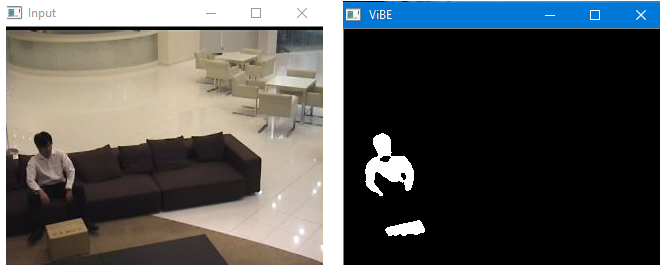
\includegraphics[scale=0.85]{img/5/stopped_example.png}
			\caption{Sekwencja \textit{sofa} z kategorii \textit{Intermittent Object Motion}}
			\label{fig:stopped_example}
	\end{figure}

	\begin{table}[h]
		\centering
		\begin{threeparttable}
			\caption{Średnie rezultaty uzyskane dla sekwencji z kategorii \textit{Intermittent Object Motion}}
			\label{tab:intermittent}
	\small{
			\begin{tabular}{| R{3cm} || m{1cm} | m{1cm} | m{1cm} | m{1cm} | m{1cm} | m{1cm} | m{1cm} |}  
			\hline
			 & \multicolumn{1}{l|}{\textit{Recall}} & \multicolumn{1}{l|}{\textit{Spec}} & \multicolumn{1}{l|}{\textit{FPR}}
			 & \multicolumn{1}{l|}{\textit{FNR}} & \multicolumn{1}{l|}{\textit{PWC}} & \multicolumn{1}{l|}{\textit{F1}} & \multicolumn{1}{l|}{\textit{Prec}} \\
			\hline \hline			
			\textit{metoda naiwna} & \num{0.7292} & \num{0.8802} & \num{0.1198} & \num{0.2708} & \num{12.1482} & \num{0.5184} & \num{0.5065} \\
			\hline
			\textit{odejmowanie ramek} & \num{0.0497} & \num{0.9986} & \num{0.0014} & \num{0.9503} & \num{6.2573} & \num{0.0869} & \num{0.8729} \\
			\hline
			\textit{średnia krocząca} & \num{0.2402} & \num{0.9817} & \num{0.0183} & \num{0.7598} & \num{6.5975} & \num{0.2903} & \num{0.4795} \\
			\hline
			\textit{ViBE} & \num{0.6338} & \num{0.9055} & \num{0.0945} & \num{0.3662} & \num{10.0766} & \num{0.4562} & \num{0.4463} \\
			\hline
            \textit{PBAS} & \num{0.1471} & \num{0.9997} & \num{0.0003} & \num{0.8529} & \num{5.6189} & \num{0.2389} & \num{0.9293} \\
			\hline
			\textit{PBAS+} & \num{0.8048} & \num{0.9868} & \num{0.0132} & \num{0.1952} & \num{2.1968} & \num{0.7778} & \num{0.7847} \\
			\hline 		
			\textit{GMM} & \num{0.3403} & \num{0.9719} & \num{0.0281} & \num{0.6597} & \num{10.2164} & \num{0.4108} & \num{0.6682} \\
			\hline
			\end{tabular}
			}		
		\end{threeparttable}
	\end{table}

Na podstawie uzyskanych wyników można zauważyć, że testowane algorytmy nie dają zbyt dobrych rezultatów. 
W większości przypadków występuje niska wartość wskaźnika \textit{recall} oraz duża wartość \textit{PWC}, co oznacza, że wiele spośród statycznych obiektów zostało wtopionych w model tła. 
Ponownie zaskakująco dużą dokładność uzyskano dla metody naiwnej.  
%%TODO no bo pewnie dlatego ze na poczatku scena była pusta
Otrzymane wskaźniki są na podobnym poziomie co te uzyskane dla algorytmu \textit{ViBE}. Taki rezultat należy jednak traktować jako przypadek, spowodowany faktem, że scena w pierwszej ramce obrazu była pusta. W rzeczywistych warunkach algorytm ten nie zapewnia zadowalających wyników.
Metody \textit{PBAS} w wersji podstawowej oraz zawierającej dodatkowy mechanizm detekcji obiektów statycznych (\textit{PBAS+}) zostały porównane niezależnie od reszty. 
Wyniki zawierające rezultaty obu algorytmów dla poszczególnych sekwencji z tej kategorii zamieszczono w tabeli \ref{tab:pbas_plus_intermittent}.

	\begin{table}[h]
		\centering
		\begin{threeparttable}
			\caption{Średnie rezultaty uzyskane dla sekwencji z kategorii \textit{Intermittent Object Motion}}
			\label{tab:pbas_plus_intermittent}
	\small{
			\begin{tabular}{| R{3cm} | m{1cm} | m{1cm} | m{1cm} | m{1cm} | m{1cm} | m{1cm} | m{1cm} | m{1cm} |}  
			\hline
			 \multicolumn{1}{|c|}{\textit{Kategoria}} & \multicolumn{1}{l|}{\textit{Algorytm}} & \multicolumn{1}{l|}{\textit{Recall}} & \multicolumn{1}{l|}{\textit{Spec}} & \multicolumn{1}{l|}{\textit{FPR}}
			 & \multicolumn{1}{l|}{\textit{FNR}} & \multicolumn{1}{l|}{\textit{PWC}} & \multicolumn{1}{l|}{\textit{F1}} & \multicolumn{1}{l|}{\textit{Prec}} \\
            \hline \hline			 
            \multirow{2}{*}{\textit{abandonedBox}} & \textit{PBAS} & \num{0.2217} & \num{0.9991} & \num{0.0009} & \num{0.7783} & \num{3.8330} & \num{0.3574} & \num{0.9224} \\
            & \textit{PBAS+} & \num{0.9879} & \num{0.9739} & \num{0.0261} & \num{0.0121} & \num{2.5427} & \num{0.7889} & \num{0.6566} \\	
            \hline
            \multirow{2}{*}{\textit{parking}} & \textit{PBAS} & \num{0.0032} & \num{1.0000} & \num{0.0000} & \num{0.9968} & \num{7.7201} & \num{0.0064} & \num{1.0000} \\
            & \textit{PBAS+} & \num{0.6120} & \num{0.9873} & \num{0.0127} & \num{0.3880} & \num{4.1770} & \num{0.6941} & \num{0.8017} \\
            \hline
            \multirow{2}{*}{\textit{sofa}} & \textit{PBAS} & \num{0.2760} & \num{0.9994} & \num{0.0006} & \num{0.7240} & \num{3.2187} & \num{0.4284} & \num{0.9562} \\
            & \textit{PBAS+} & \num{0.5898} & \num{0.9967} & \num{0.0033} & \num{0.4102} & \num{2.1043} & \num{0.7101} & \num{0.8921} \\
            \hline
            \multirow{2}{*}{\textit{streetLight}} & \textit{PBAS} & \num{0.0421} & \num{1.0000} & \num{0.0000} & \num{0.9579} & \num{4.6503} & \num{0.0808} & \num{0.9999} \\
            & \textit{PBAS+} & \num{0.9590} & \num{0.9999} & \num{0.0001} & \num{0.0410} & \num{0.2093} & \num{0.9780} & \num{0.9978} \\
            \hline
            \multirow{2}{*}{\textit{tramstop}} & \textit{PBAS} & \num{0.2442} & \num{0.9998} & \num{0.0002} & \num{0.7558} & \num{13.5829} & \num{0.3922} & \num{0.9966} \\
            & \textit{PBAS+} & \num{0.9558} & \num{0.9685} & \num{0.0315} & \num{0.0442} & \num{3.3774} & \num{0.9104} & \num{0.8691} \\
            \hline
            \multirow{2}{*}{\textit{winterDriveway}} & \textit{PBAS} & \num{0.0954} & \num{0.9997} & \num{0.0003} & \num{0.9046} & \num{0.7083} & \num{0.1679} & \num{0.7008} \\
            & \textit{PBAS+} & \num{0.7245} & \num{0.9943} & \num{0.0057} & \num{0.2755} & \num{0.7700} & \num{0.5851} & \num{0.4906} \\
            \hline
            \multirow{2}{*}{\textbf{średnia}} & \textbf{\textit{PBAS}} & \textbf{\num{0.1471}} & \textbf{\num{0.9997}} & \textbf{\num{0.0003}} & \textbf{\num{0.8529}} & \textbf{\num{5.6189}} & \textbf{\num{0.2389}} & \textbf{\num{0.9293}} \\
            & \textbf{\textit{PBAS+}} & \textbf{\num{0.8048}} & \textbf{\num{0.9868}} & \textbf{\num{0.0132}} & \textbf{\num{0.1952}} & \textbf{\num{2.1968}} & \textbf{\num{0.7778}} & \textbf{\num{0.7847}} \\
            \hline
			\end{tabular}
			}		
		\end{threeparttable}
	\end{table}

Po dokonaniu analizy otrzymanych wyników można śmiało stwierdzić, że zaimplementowany mechanizm spełnia swoje zadanie. 
Rezultaty osiągnięte przez algorytm \textit{PBAS+} są zdecydowanie lepsze niż innych algorytmów, dodatkowo widać olbrzymią poprawę w stosunku do standardowej wersji tej metody. 
Należy zaznaczyć, że w niektórych przypadkach statyczny obiekt umieszczony był daleko od kamery, na drugim planie. Skutkowało to jego niewielkim rozmiarem co stanowiło dodatkowe utrudnienie dla algorytmu.
%%TODO co to znaczy daleko w tle ? że był o niewielkim rozmiarze ?
Przykładem takiej sekwencji jest \textit{parking}. 
Mimo takich utrudnień uzyskany wyniki można uznać za zadowalający. 
Drugą bardzo skomplikowaną do analizy sekwencją jest \textit{sofa}, gdzie za największą trudność należy uznać zbliżoną kolorystykę obiektów. 
W~przypadku sekwencji \textit{winterDriveway} wpływ na gorszy niż w pozostałych testach wynik, miały głownie bardzo trudne warunki pogodowe w których film ten został nagramy. 


\subsection{Kamera termowizyjna}
\label{subsec:kamera_termowizyjna}

W kategorii \textit{Thermal} zawiera się 5 sekwencji, do których nagrania wykorzystano kamerę pracującą w paśmie podczerwieni. 
Przykładowy kadr z takiej sekwencji zamieszczono na rysunku \ref{fig:thermal_example}. 
Głównymi trudnościami w tego typu obrazach jest słaby kontrast pomiędzy obiektami oraz różnego rodzaju odbicia cieplne np. oknie lub na podłodze.
Wyniki przeprowadzonych testów dla poszczególnych algorytmów zamieszczono w tabeli \ref{tab:thermal}.

    \begin{figure}[h]
			\centering
			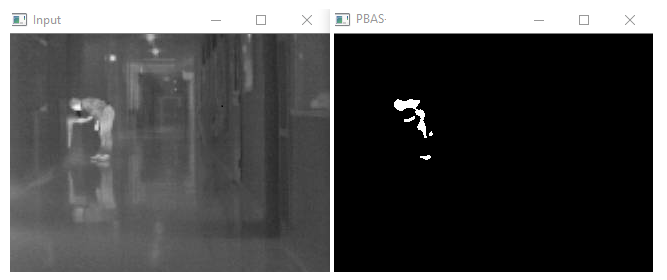
\includegraphics[scale=0.85]{img/5/thermal_example.png}
			\caption{Sekwencja \textit{corridor} z kategorii\textit{Thermal}}
			\label{fig:thermal_example}
	\end{figure}

	\begin{table}[h]
		\centering
		\begin{threeparttable}
			\caption{Średnie rezultaty uzyskane dla sekwencji z kategorii \textit{Thermal}}
			\label{tab:thermal}
	\small{
			\begin{tabular}{| R{3cm} || m{1cm} | m{1cm} | m{1cm} | m{1cm} | m{1cm} | m{1cm} | m{1cm} |}  
			\hline
			 & \multicolumn{1}{l|}{\textit{Recall}} & \multicolumn{1}{l|}{\textit{Spec}} & \multicolumn{1}{l|}{\textit{FPR}}
			 & \multicolumn{1}{l|}{\textit{FNR}} & \multicolumn{1}{l|}{\textit{PWC}} & \multicolumn{1}{l|}{\textit{F1}} & \multicolumn{1}{l|}{\textit{Prec}} \\
			\hline \hline
			\textit{metoda naiwna} & \num{0.6396} & \num{0.9936} & \num{0.0064} & \num{0.3604} & \num{1.9062} & \num{0.6982} & \num{0.8189} \\
			\hline
			\textit{odejmowanie ramek} & \num{0.0812} & \num{0.9997} & \num{0.0003} & \num{0.9188} & \num{6.7849} & \num{0.1283} & \num{0.9158} \\
			\hline
			\textit{średnia krocząca} & \num{0.3447} & \num{0.9933} & \num{0.0067} & \num{0.6553} & \num{5.8723} & \num{0.4238} & \num{0.7338} \\
			\hline
			\textit{ViBE} & \num{0.2772} & \num{0.9930} & \num{0.0070} & \num{0.7228} & \num{5.2324} & \num{0.3936} & \num{0.7555} \\
			\hline
            \textit{PBAS} & \num{0.2737} & \num{0.9980} & \num{0.0020} & \num{0.7263} & \num{5.3672} & \num{0.4005} & \num{0.9489} \\
			\hline
			\textit{PBAS+} & \num{0.4236} & \num{0.9976} & \num{0.0024} & \num{0.5764} & \num{4.8207} & \num{0.5507} & \num{0.8981} \\
			\hline 		
			\textit{GMM} & \num{0.3563} & \num{0.9983} & \num{0.0017} & \num{0.6415} & \num{5.5093} & \num{0.5041} & \num{0.9374} \\
			\hline
			\end{tabular}
			}		
		\end{threeparttable}
	\end{table}

Uzyskane wyniki pokazują, że w przypadku tej kategorii, większą trudnością jest identyfikacja obiektów. 
Rzadko występują przypadki, kiedy element tła zostanie błędnie zaklasyfikowany jako pierwszy plan. 
Świadczy o tym dość wysoka wartość wskaźników \textit{spec} i \textit{prec} dla wszystkich algorytmów. 
Niestety w większości przypadków nie udało się rozpoznać znacznej lliczby obiektów, rezultatem tego są niskie wartości wskaźnika \textit{recall}. 

\subsection{Podsumowanie}
\label{subsec:testy_podsumowanie}

Tabela \ref{tab:total_avg} zawiera zestawienie uśrednionych wyników dla poszczególnych algorytmów. 
Dla każdej metody możemy zaobserwować wysoką wartość wskaźnika \textit{spec}, oznacza to dobrą dokładność przy rozpoznawaniu pikseli będących elementami tła. 
Taki wynik jest przewidywalny, gdyż pikseli reprezentujących tło jest w większości przypadków zdecydowanie więcej niż pierwszoplanowych. 
Niestety dużo częściej występującym zjawiskiem jest zakwalifikowanie piksela będącego elementem pierwszego planu jako tła, sytuacja odwrotna zdarza się zdecydowanie rzadziej. 
Dla każdego algorytmu wartość wskaźnika \textit{prec} jest wyraźnie niższa niż wartość \textit{spec}, taki rezultat potwierdza omówione zjawisko. 

	\begin{table}[h]
		\centering
		\begin{threeparttable}
			\caption{Średnie rezultaty uzyskane dla poszczególnych algorytmów}
			\label{tab:total_avg}
	\small{
			\begin{tabular}{| R{3cm} || m{1cm} | m{1cm} | m{1cm} | m{1cm} | m{1cm} | m{1cm} | m{1cm} |}  
			\hline
			 & \multicolumn{1}{l|}{\textit{Recall}} & \multicolumn{1}{l|}{\textit{Spec}} & \multicolumn{1}{l|}{\textit{FPR}}
			 & \multicolumn{1}{l|}{\textit{FNR}} & \multicolumn{1}{l|}{\textit{PWC}} & \multicolumn{1}{l|}{\textit{F1}} & \multicolumn{1}{l|}{\textit{Prec}} \\
			\hline \hline
			\textit{metoda naiwna} & \num{0.7560} & \num{0.9424} & \num{0.0576} & \num{0.2440} & \num{6.2653} & \num{0.5735} & \num{0.5562} \\
			\hline
			\textit{odejmowanie ramek} & \num{0.2195} & \num{0.9766} & \num{0.0234} & \num{0.7805} & \num{5.9806} & \num{0.2226} & \num{0.6963} \\
			\hline
			\textit{średnia krocząca} & \num{0.5466} & \num{0.9532} & \num{0.0468} & \num{0.4534} & \num{6.9666} & \num{0.3891} & \num{0.4323} \\
			\hline
			\textit{ViBE} & \num{0.7056} & \num{0.9683} & \num{0.0317} & \num{0.2944} & \num{4.2938} & \num{0.6268} & \num{0.6670} \\
			\hline
            \textit{PBAS} & \num{0.4848} & \num{0.9944} & \num{0.0056} & \num{0.5152} & \num{3.1042} & \num{0.5493} & \num{0.8333} \\
			\hline
			\textit{PBAS+} & \num{0.8042} & \num{0.9721} & \num{0.0279} & \num{0.1958} & \num{3.8507} & \num{0.6741} & \num{0.6917} \\
			\hline 		
			\textit{GMM} & \num{0.4940} & \num{0.9693} & \num{0.0307} & \num{0.5056} & \num{6.4052} & \num{0.4932} & \num{0.6491} \\
			\hline
			\end{tabular}
			}		
		\end{threeparttable}
	\end{table}
	
Jak zostało już wielokrotnie zaznaczone przy opisie poszczególnych kategorii sekwencji testowych, stosunkowo dobre wyniki uzyskano dla metody naiwnej. 
Otrzymane wartości wskaźniki jakości są zdecydowanie wyższe niż w przypadku pozostałych prostych algorytmów. 
Zdecydowanie najlepiej z sekwencjami testowymi poradził sobie algorytm \textit{PBAS} z dodatkowym mechanizmem detekcji obiektów statycznych.
Uzyskano wysoki procent rozpoznanych obiektów pierwszoplanowych (parametr \textit{recall}), przy zachowaniu dobrej dokładności i niewielkim procencie źle rozpoznanych pikseli (parametry \textit{prec} i \textit{PWC}). 
Takie wyniki oznaczają, że mechanizm indeksacji, połączony z analizą krawędzi poprawia jakość detekcji nie tylko w przypadku obiektów statycznych. 

Kolejną wartą uwagi obserwacją jest fakt, że standardowa wersja algorytmu \textit{PBAS}, osiąga słabsze wyniki od metody \textit{ViBE}, mimo że teoretycznie jest jej bardziej rozbudowaną wersją. %%TODO 1. styl, dwa słabsze niż ViBE ? ale tak jest w changedetection ?? przecież nie... choć oni tam coś kombinowali z tym PBAS'em
Dodatkowe manipulowanie progiem przynależności i prawdopodobieństwem aktualizacji nie zawsze wpływa pozytywnie na wynik końcowy. 
Rozczarowujące są również rezultaty otrzymane dla algorytmu \textit{GMM}, szczególnie widoczny jest bardzo wysoki procent źle sklasyfikowanych pikseli \textit{PWC} oraz słaba rozpoznawalność obiektów pierwszoplanowych (parametr \textit{recall}).

Niestety rozszerzona wersja algorytmu \textit{ViBE}, zawierająca dodatkowy mechanizm redukcji ruchu kamery, nie sprawdziła się w testach z wykorzystaniem sekwencji testowych. 
Autorzy publikacji \cite{kryjak_14_vibe} z której pochodzi metoda zaproponowali alternatywny sposób przetestowania metody w rzeczywistym środowisku, jedynie z wykorzystaniem ruchomej, nie drgającej kamery. 
Uzyskane w tak przeprowadzonym badaniu rezultaty dały bardzo obiecujące wyniki.
%TODO no ale PAn tych wyników już nie powtarzał...


W porównaniu do metod zaprezentowanych w innych publikacjach, wyniki najlepszego z zaimplementowanych algorytmów (\textit{PBAS+}) można uznać za zadowalające. 
Zaprezentowana w publikacji \cite{wang_14} metoda \textit{FTSG} osiąga co prawda zdecydowanie lepsze rezultaty, jednak należy pamiętać, że zawiera ona wiele dodatkowych mechanizmów takich jak na przykład wykrywanie dynamicznego tła. 
Rezultaty wersji \textit{GMM} przedstawionej w \cite{} są bardzo zbliżone do wyników implementacji, która została przedstawiona w niniejszej pracy.
%TODO brak odnośnika